\documentclass[a4paper,12pt]{article}

%%% Работа с русским языком
\usepackage{cmap}					% поиск в PDF
\usepackage{mathtext} 				% русские буквы в формулах
\usepackage[T2A]{fontenc}			% кодировка
\usepackage[utf8]{inputenc}			% кодировка исходного текста
\usepackage[english,russian]{babel}	% локализация и переносы

%%% Страница
\usepackage{extsizes} % Возможность сделать 14-й шрифт
\usepackage{geometry} % Создание полей
\geometry{top = 2.5cm}
\geometry{bottom = 2cm}
\geometry{left = 3cm}
\geometry{right = 1.5cm}
\renewcommand{\baselinestretch}{1.5} % Интерлиньяж 1.5

%%% Дополнительная работа с математикой
\usepackage{amsmath,amsfonts,amssymb,amsthm,mathtools} % AMS
\usepackage{icomma} % "Умная" запятая: $0,2$ --- число, $0, 2$ --- перечисление

%% Номера формул
%\mathtoolsset{showonlyrefs=true} % Показывать номера только у тех формул, на которые есть \eqref{} в тексте.
%\usepackage{leqno} % Нумерация формул слева

%% Свои команды
\DeclareMathOperator{\sgn}{\mathop{sgn}}

%% Перенос знаков в формулах (по Львовскому)
\newcommand*{\hm}[1]{#1\nobreak\discretionary{}
	{\hbox{$\mathsurround=0pt #1$}}{}}

%%% Работа с картинками
\usepackage{graphicx}  % Для вставки рисунков
\graphicspath{{images/}{images2/}}  % папки с картинками
\setlength\fboxsep{3pt} % Отступ рамки \fbox{} от рисунка
\setlength\fboxrule{1pt} % Толщина линий рамки \fbox{}
\usepackage{wrapfig} % Обтекание рисунков текстом

%%% Работа с таблицами
\usepackage{array,tabularx,tabulary,booktabs} % Дополнительная работа с таблицами
\usepackage{longtable}  % Длинные таблицы
\usepackage{multirow} % Слияние строк в таблице

%%% Теоремы
\theoremstyle{plain} % Стиль по умолчанию
\newtheorem{theorem}{Теорема}[section]
\newtheorem{proposition}[theorem]{Утверждение}

\theoremstyle{definition} % "Определение"
\newtheorem{corollary}{Следствие}[theorem]
\newtheorem{problem}{Задача}[section]

\theoremstyle{remark} % "Примечание"
\newtheorem*{nonum}{Решение}

%%% Программирование
\usepackage{etoolbox} % логические операторы

\usepackage{lastpage} % Узнать, сколько всего страниц в документе.

\usepackage{soul} % Модификаторы начертания

\usepackage{graphicx} %Подключаю модули для добавления картинок
\graphicspath{.}
\DeclareGraphicsExtensions{.pdf,.png,.jpg}
	
	\renewcommand{\baselinestretch}{1.5}
	
\begin{document}
\renewcommand{\contentsname}{\Large Содержание}
\renewcommand{\bibname}{\normalfont\Large\bfseries Список литературы}

\begin{titlepage}
	\begin{center}
		Министерство науки и высшего образования Российской Федерации \\
		НАЦИОНАЛЬНЫЙ ИССЛЕДОВАТЕЛЬСКИЙ ЯДЕРНЫЙ УНИВЕРСИТЕТ <<МИФИ>> \\*
		\hrulefill
	\end{center}
	
	\begin{center}
		ИНСТИТУТ ЛАЗЕРНЫХ И ПЛАЗМЕННЫХ ТЕХНОЛОГИЙ\\
		КАФЕДРА №31 ПРИКЛАДНАЯ МАТЕМАТИКА
	\end{center}
	\vspace{1cm}
	
	\vspace{2em}
	
	\begin{center}
		\large{Отчет}
		
		по научно-исследовательской работе на тему:
	\end{center}
	\begin{center}
		\large <<Оптимизация канального радиатора>>
	\end{center}
	\begin{center}
		\large \textit{Выполнил: Есис А. И.}
		
		\textit{Руководитель проекта: Чмыхов М. А.}
	\end{center}
	
	
	\vspace{22em}
	
	\begin{center}
		г. Москва 2023
	\end{center}
\end{titlepage}

\newpage
\section*{Аннотация}

Данная работа посвящена исследованию и оптимизации формы радиатора с применением трех программных инструментов: OpenFOAM, ParaView и SALOME Meca. Целью исследования является повышение эффективности радиатора путем оптимизации его геометрии.

В начале исследования используется SALOME Meca для построения геометрии и сетки радиатора. На втором этапе проводятся численные симуляции с использованием OpenFOAM. В результате симуляций получаются данные о тепловом и газодинамическом поведении радиатора. Наконец, результаты численных симуляций визуализируются с помощью ParaView. И делается вывод о наиболее оптимальной форме радиатора.

\newpage 
\tableofcontents
\setcounter{page}{3}

\newpage
\section{Введение}


OpenFOAM, ParaView и SALOME Meca являются мощными программными инструментами, широко применяемыми в области вычислительной гидрогазодинамики (CFD) и численного моделирования. Вместе они предоставляют комплексное решение для анализа и визуализации сложных физических процессов, таких как течение жидкостей, теплообмен, движение твердых тел и другие.

OpenFOAM (Open Field Operation and Manipulation) является свободным и открытым программным обеспечением для решения уравнений Навье-Стокса и других математических моделей, связанных с течением жидкостей и газов. OpenFOAM предоставляет широкий спектр методов решения, таких как конечно-разностные, конечно-объемные и конечно-элементные, что позволяет исследовать различные типы потоков и применять разные физические модели. Будучи свободно распространяемым и расширяемым, OpenFOAM предоставляет возможность настраивать и адаптировать код под конкретные задачи и требования.

ParaView является инструментом, который позволяет визуализировать результаты численных симуляций. Он предоставляет широкий спектр функций для создания визуализаций, включая 2D и 3D графику, построение контуров, срезов и анимаций. ParaView также поддерживает интерактивное взаимодействие с моделью, что позволяет анализировать данные в реальном времени, изменять параметры симуляции и осуществлять глубокий анализ результатов.

SALOME Meca является интегрированной средой для предварительной обработки геометрии и настройки расчетной сетки для OpenFOAM. Он предоставляет интуитивный пользовательский интерфейс, который облегчает создание и манипулирование сложными геометрическими моделями, а также настройку сеток с различной структурой. SALOME Meca также предлагает набор инструментов для проверки качества сетки и подготовки ее к последующим симуляциям в OpenFOAM \cite{wOfDocSalome}.

Вместе OpenFOAM, ParaView и SALOME Meca образуют мощный комплект инструментов для моделирования и визуализации в области вычислительной гидрогазодинамики. Они предоставляют возможность проводить сложные численные симуляции, анализировать результаты и визуализировать данные, что помогает в понимании физических процессов и принятии информированных решений в различных областях, таких как авиация, автомобильная промышленность, энергетика и многое другое.

\newpage
\section{Основная часть}

В данном проекте исследуется задача охлаждения нагретого тела с помощью установки радиатора.

В начале проекта геометрия радиатора строится с использованием графического интерфейса SALOME. Используя интуитивно понятный пользовательский интерфейс, создается геометрия радиатора. Этот этап позволяет получить исходную геометрию, которая будет использоваться для последующих анализов.

Затем, для повышения гибкости и автоматизации процесса, создается скрипт на языке Python, который генерирует геометрию радиатора. В этом скрипте можно устанавливать параметры радиатора, такие как расположение элементов. Это позволяет быстро создавать и изменять различные варианты геометрии радиатора для дальнейшего анализа и оптимизации.

Для исследования были использованы три различных варианта геометрии радиатора.
Примеры геометрии:
\begin{figure}[h]
	\begin{center}
		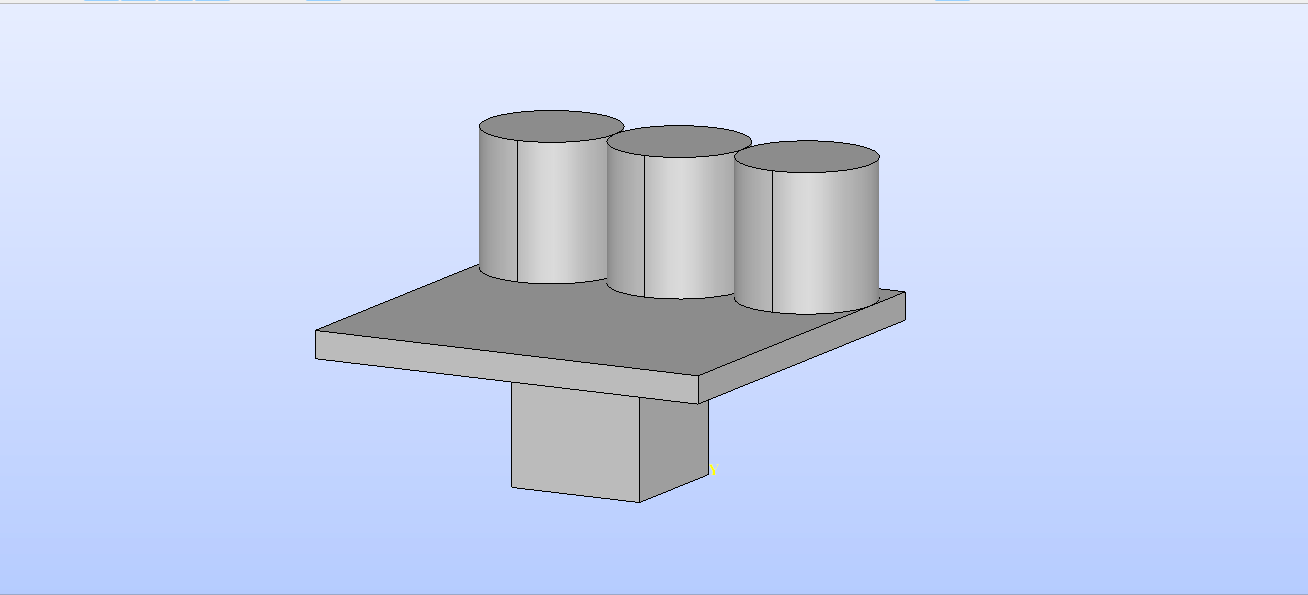
\includegraphics[width=0.5\linewidth]{1.1.png}
		\caption{Модель геометрии 1} %% подпись к рисунку
	\end{center}
\end{figure}
\begin{figure}[h]
	\begin{center}
		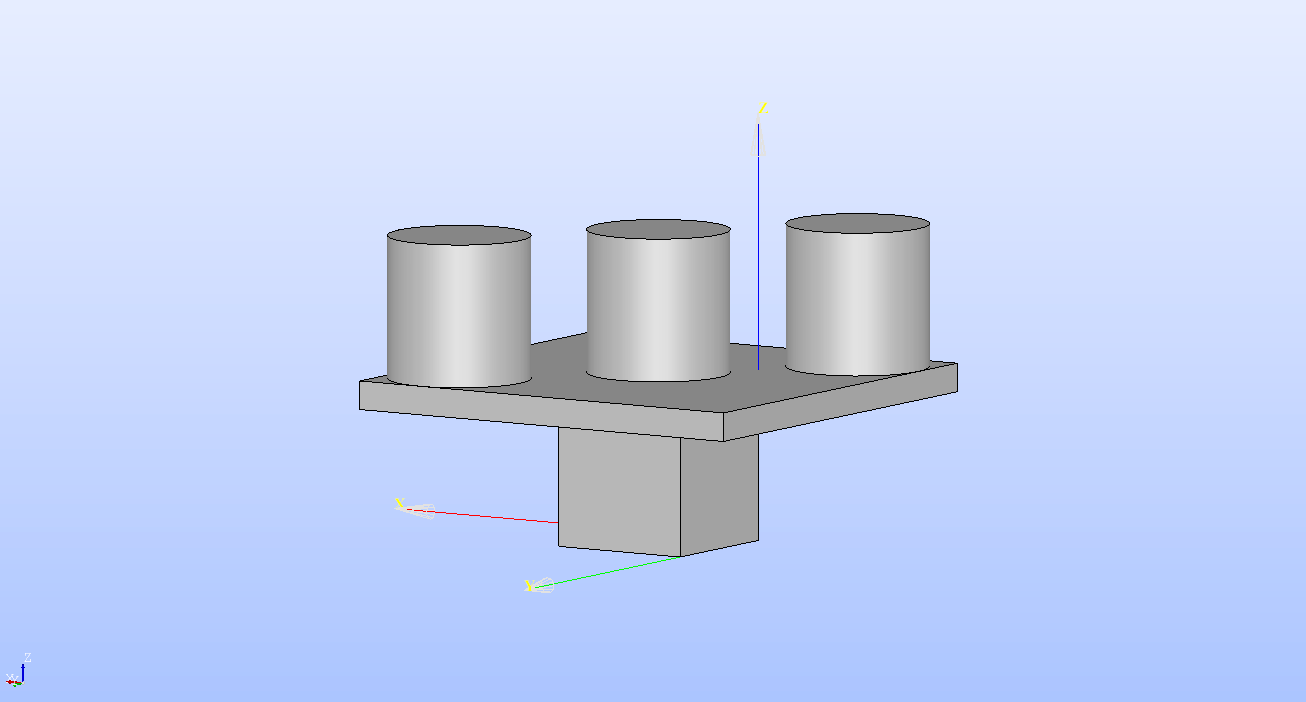
\includegraphics[width=0.5\linewidth]{1.2.png}
		\caption{Модель геометрии 2}
	\end{center}
\end{figure}
\begin{figure}[h]
	\begin{center}
		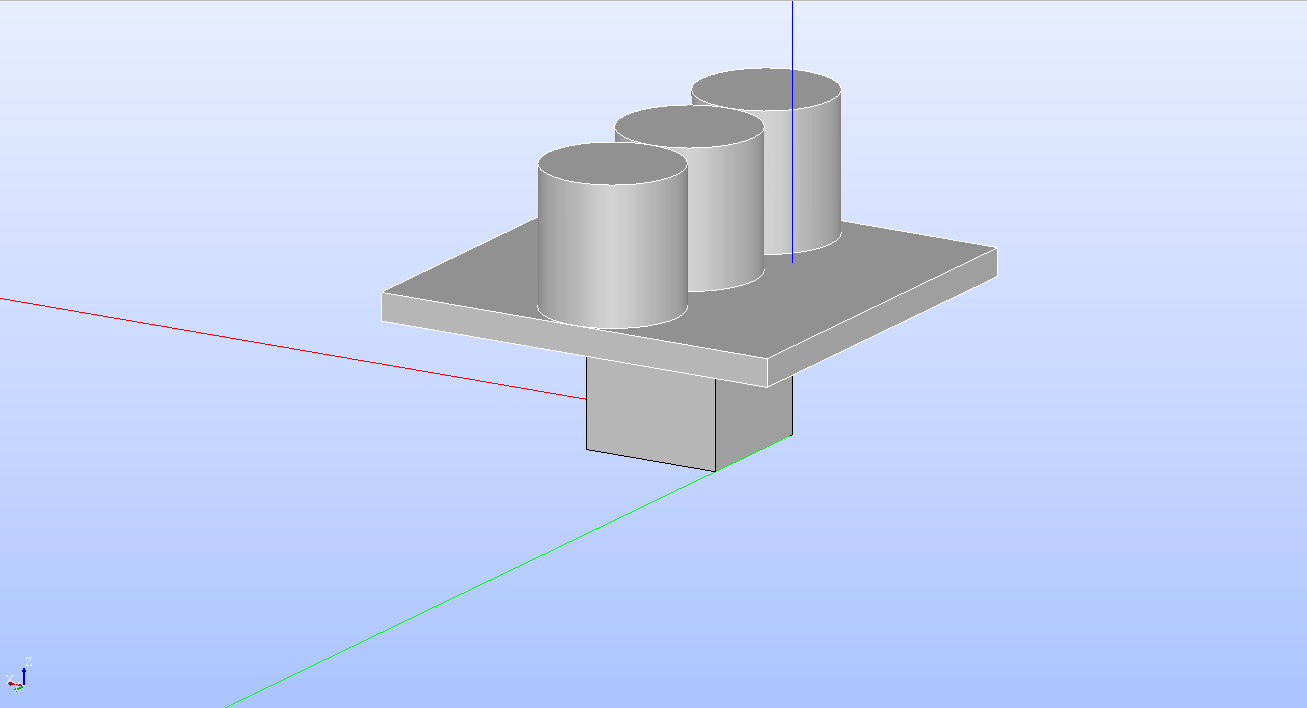
\includegraphics[width=0.5\linewidth]{1.3.png}
		\caption{Модель геометрии 3}
	\end{center}
\end{figure}
\newpage

\begin{figure}[h]
	\begin{center}
		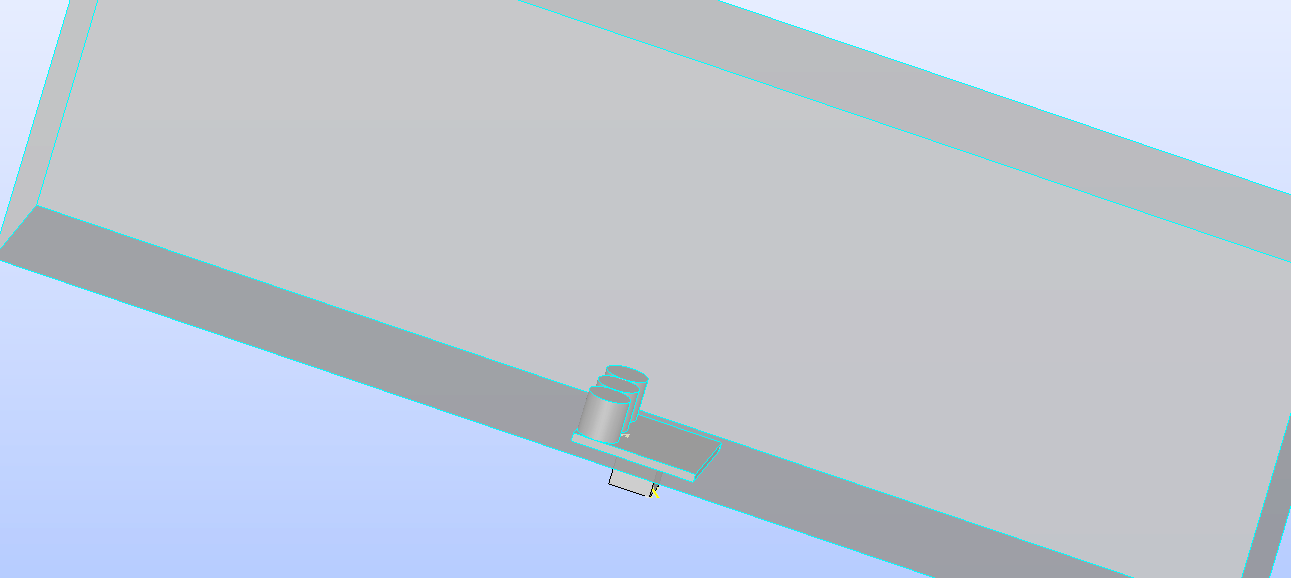
\includegraphics[width=0.5\linewidth]{2.1.png}
		\caption{Модель геометрии 1} %% подпись к рисунку
	\end{center}
\end{figure}
\begin{figure}[h]
	\begin{center}
		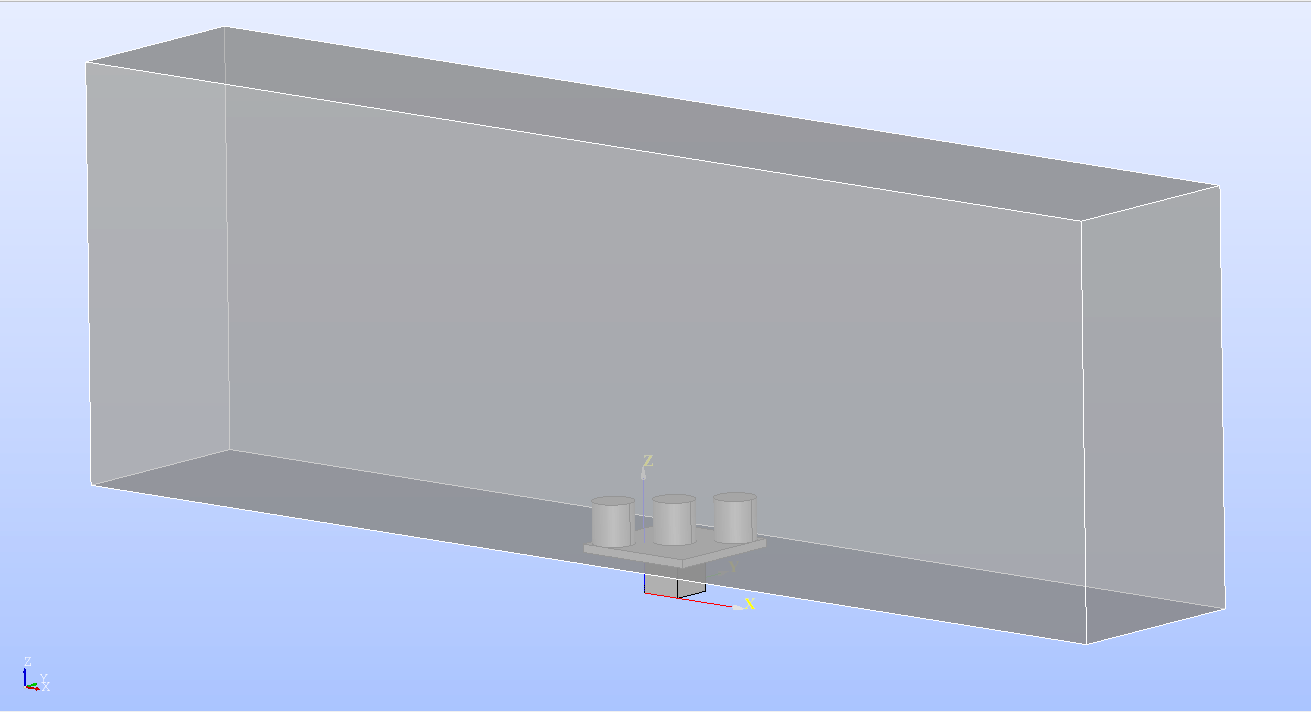
\includegraphics[width=0.5\linewidth]{2.2.png}
		\caption{Модель геометрии 2}
	\end{center}
\end{figure}
\newpage
\begin{figure}[h]
	\begin{center}
		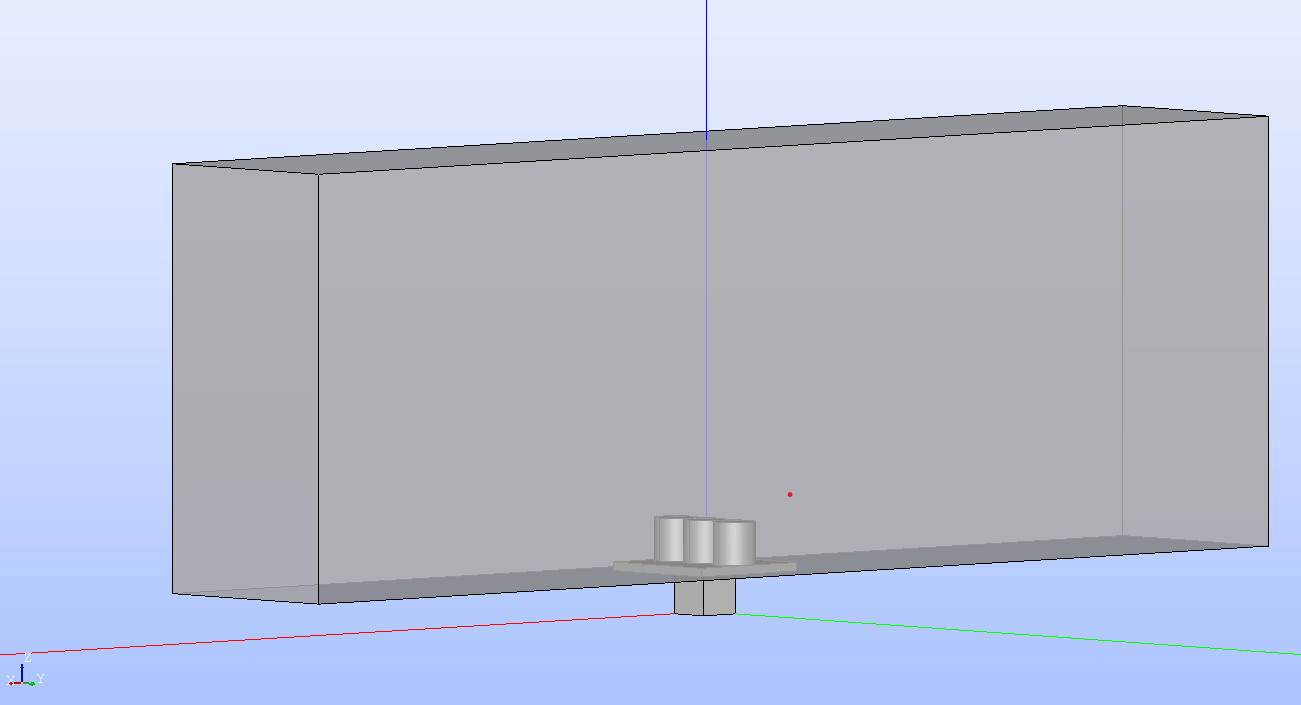
\includegraphics[width=0.5\linewidth]{2.3.png}
		\caption{Модель геометрии 3}
	\end{center}
\end{figure}

\par
В данных моделях части радиатора (3 цилиндрических элемента) являются подвижными и могут быть сдвинуты по оси Ox. Их радиус основания равен 5 мм, а высота 10 мм. 
Размеры подложки радиатора по ширине и длине 30 мм, а по высоте 2 мм. Нагреватель представляет собой куб с длиной ребра 10 мм и объемной плотностью источников тепла 2.94 * $10^7$ Вт/$м^3$. 
Скорость потока воздуха 5.6 м/с. Воздух находится в параллелепипеде размерами 300 мм по длине, 50 мм по ширине и 100 мм по высоте. Начальная температура –296.9 К. Параметры материалов приведены в таблице 1 \cite{aHeatTranserf}.

\begin{table}[h]
	\begin{tabular}{|l|l|l|l|}
		\hline
		                                          & Нагреватель & Радиатор & Воздух        \\
		Плотность {[}кг/$м^3${]}                  & 1280        & 2700     & 1.196         \\
		\hline
		Cp   {[}Дж/кг*К{]}                        & 1004        & 900      & 1005          \\
		\hline
		Коэффициент теплопроводности {[}Вт/м*К{]} & 80          & 200      &               \\
		\hline
		Молекулярная масса {[}г/моль{]}           & 50          & 27       & 28.9          \\
		\hline
		Вязкость {[}кг/м*с{]}                     &             &          & $1.8*10^{-5}$ \\
		\hline
		Число Прандтля                            &             &          & 0.7           \\
		\hline
	\end{tabular}
	\caption{Параметры задачи} %% подпись к рисунку
\end{table}

Затем по модели была построена сетка c уплотнением в области радиатора и нагревателя и произведено разбиение на регионы:

\begin{figure}[h]
	\begin{center}
		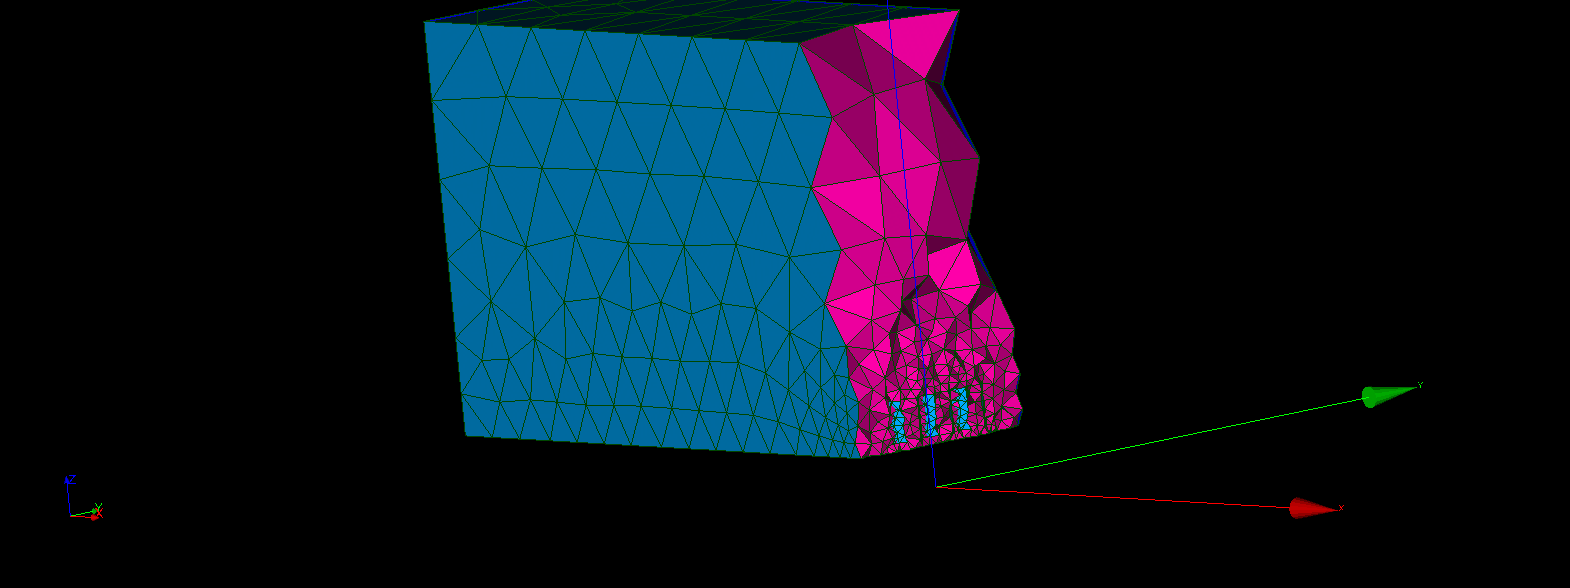
\includegraphics[width=0.35\linewidth]{3.png}
		\caption{Сетка модели 1} %% подпись к рисунку
	\end{center}
\end{figure}

\par
Для численного решения задачи используется решатель chtMultiRegionFoam.
Он применяется для расчета теплообмена между жидкостью/газом и твердым телом. А также для моделирования сложных задач, связанных с теплопередачей и теплообменом в многорегиональных системах \cite{wChtMultiRegionFoam}.
Для каждого региона задавались начальные и граничные условия. Были также заданы дополнительные функции для анализа \cite{aHeatTranserf}.
Для моделей были получены следующие результаты распределений по температурам:

\begin{figure}[h]
	\begin{center}
		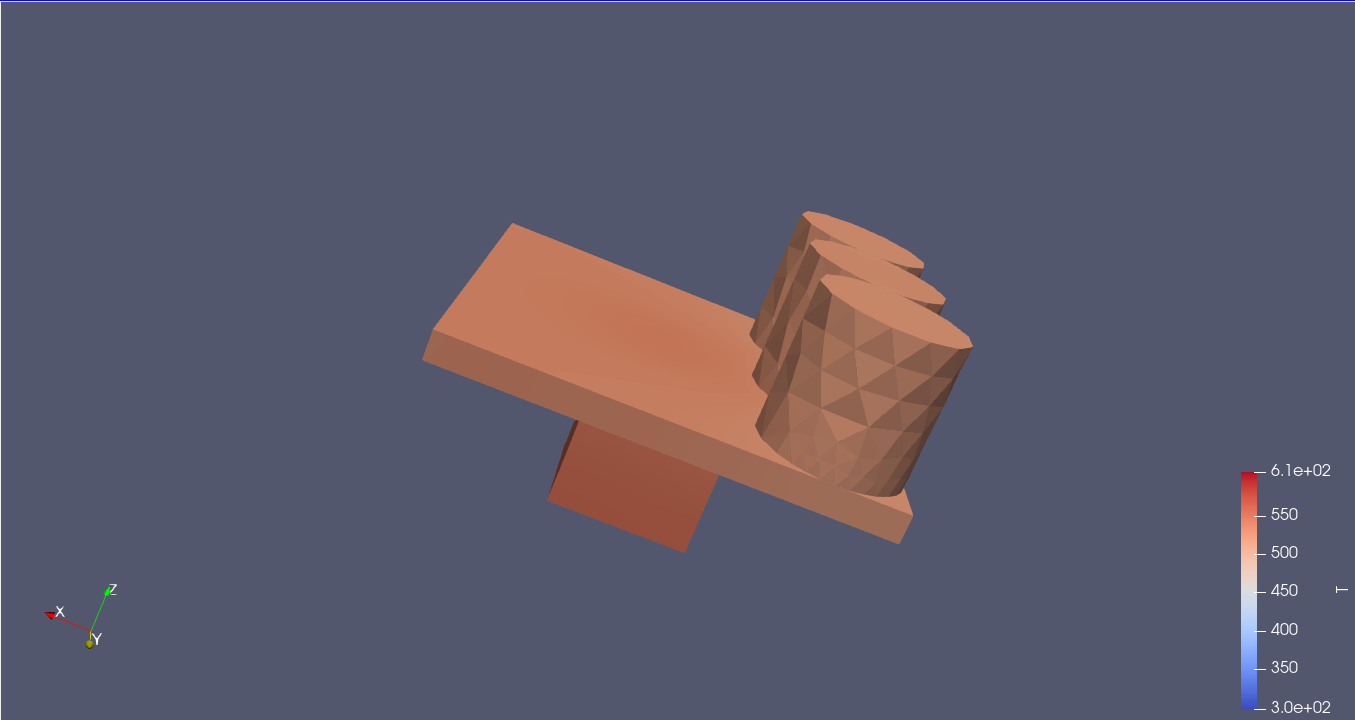
\includegraphics[width=0.45\linewidth]{5.1.png}
		\caption{Распределение температуры для модели 1} %% подпись к рисунку
	\end{center}
\end{figure}

\begin{figure}[h]
	\begin{center}
		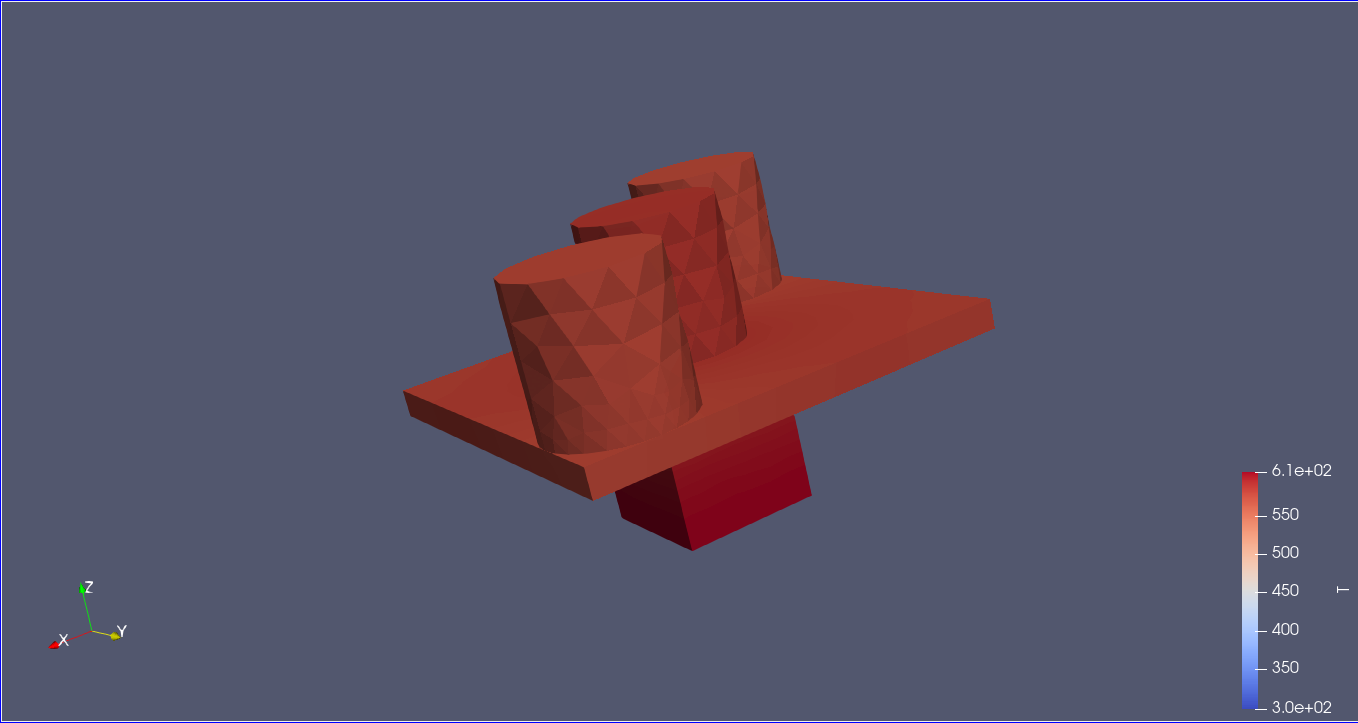
\includegraphics[width=0.45\linewidth]{5.2.png}
		\caption{Распределение температуры для модели 2} %% подпись к рисунку
	\end{center}
\end{figure}

\begin{figure}[h]
	\begin{center}
		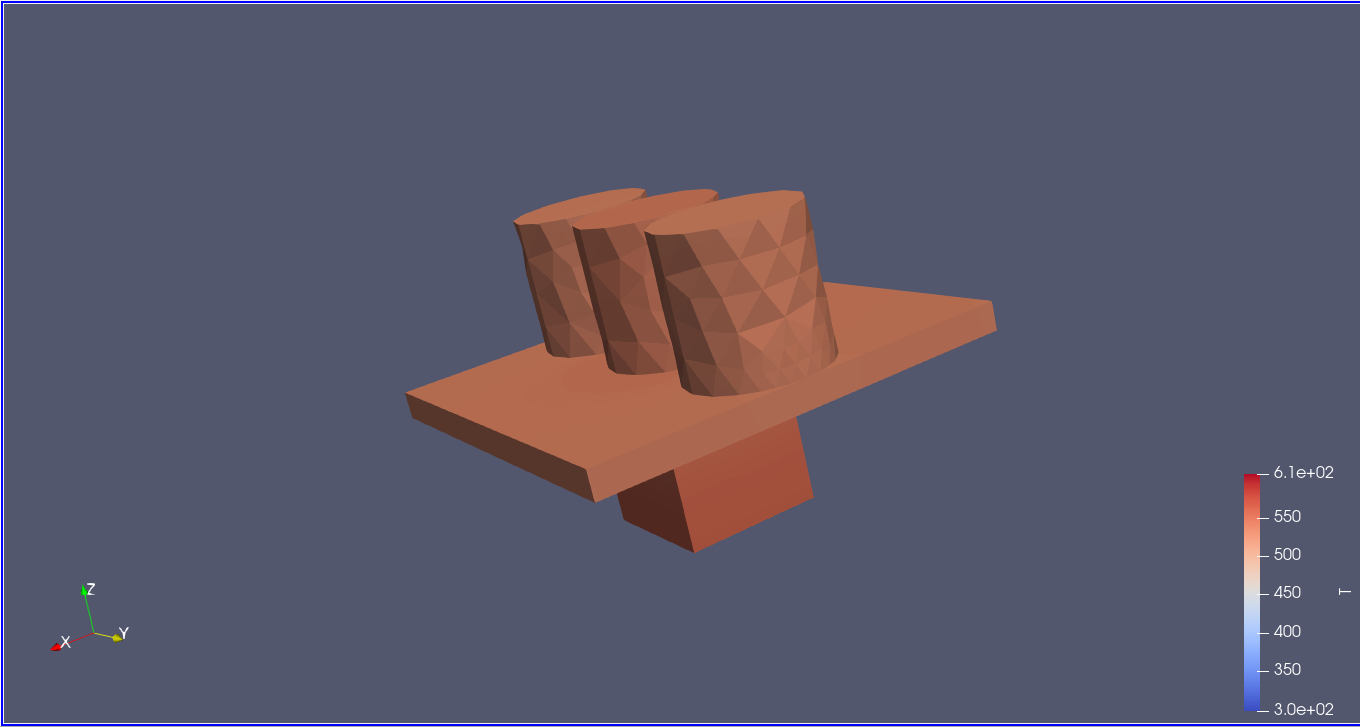
\includegraphics[width=0.45\linewidth]{5.3.png}
		\caption{Распределение температуры для модели 3} %% подпись к рисунку
	\end{center}
\end{figure}

\newpage
Были получены следующие результаты для моделей:
\begin{enumerate}
	\item \textbf{Первая модель:}
	      \begin{itemize}
		      \item Средняя температура радиатора: 508.381 К
		      \item Средняя температура нагревателя: 533.363 К
		      \item Средняя температура интерфейса между нагревателем и радиатором: 521.537 К
	      \end{itemize}
	\item \textbf{Вторая модель:}
	      \begin{itemize}
		      \item Средняя температура радиатора: 555.23 К
		      \item Средняя температура нагревателя: 576.306 К
		      \item Средняя температура интерфейса между нагревателем и радиатором: 564.451 К
	      \end{itemize}
	\item \textbf{Третья модель:}
	      \begin{itemize}
		      \item Средняя температура радиатора: 519.325 К
		      \item Средняя температура нагревателя: 537.741 К
		      \item Средняя температура интерфейса между нагревателем и радиатором: 525.862 К
	      \end{itemize}
\end{enumerate}

Построены графики температуры в нагревателе:
\newpage
\begin{figure}[h]
	\begin{center}
		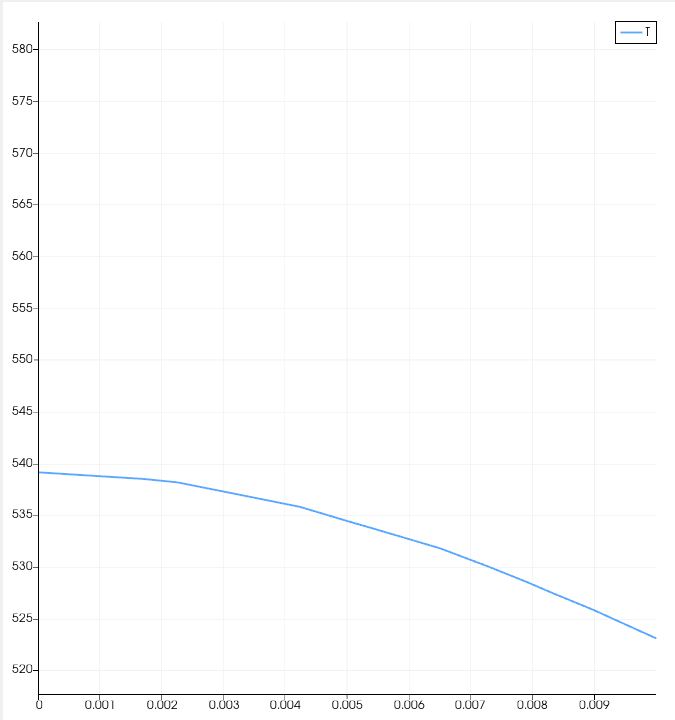
\includegraphics[width=0.4\linewidth]{6.1.png}
		\caption{Распределение температуры в нагревателе для модели 1} %% подпись к рисунку
	\end{center}
\end{figure}
\begin{figure}[h]
	\begin{center}
		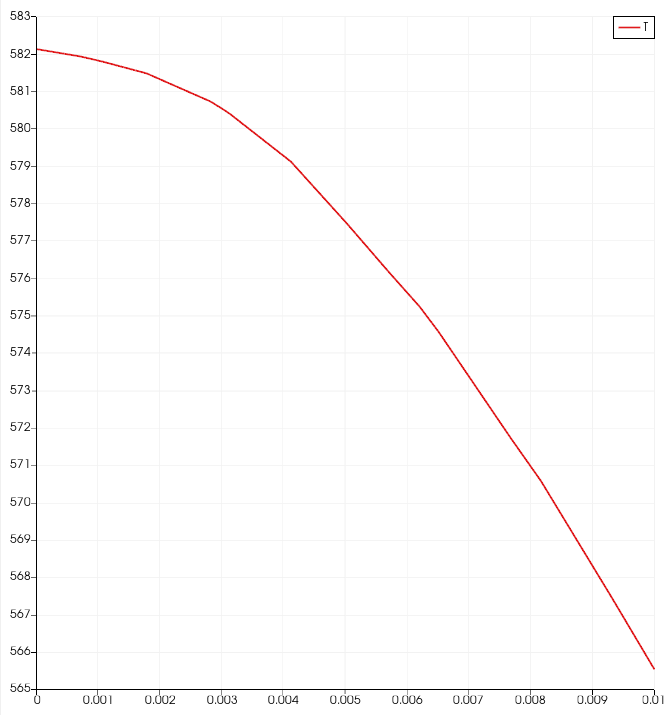
\includegraphics[width=0.4\linewidth]{6.2.png}
		\caption{Распределение температуры в нагревателе для модели 2} %% подпись к рисунку
	\end{center}
\end{figure}
\newpage
\begin{figure}[h]
	\begin{center}
		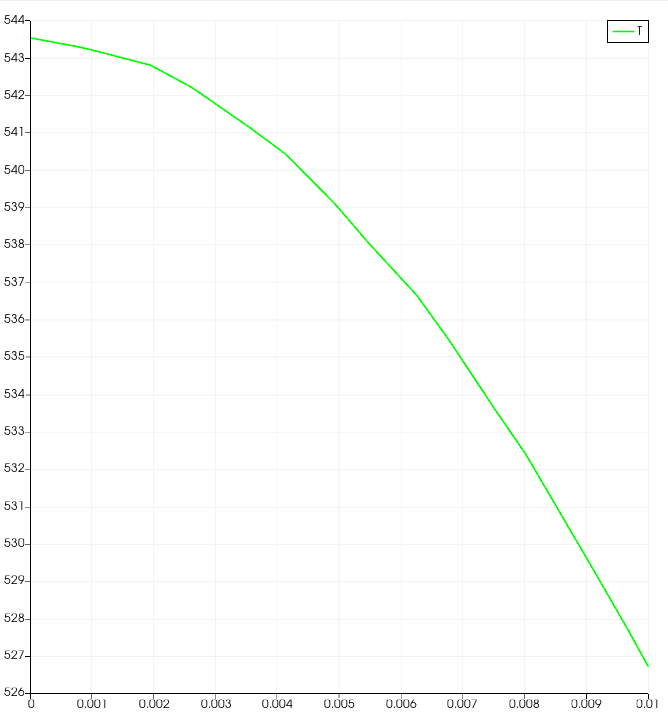
\includegraphics[width=0.4\linewidth]{6.3.png}
		\caption{Распределение температуры в нагревателе для модели 3} %% подпись к рисунку
	\end{center}
\end{figure}
\begin{figure}[h]
	\begin{center}
		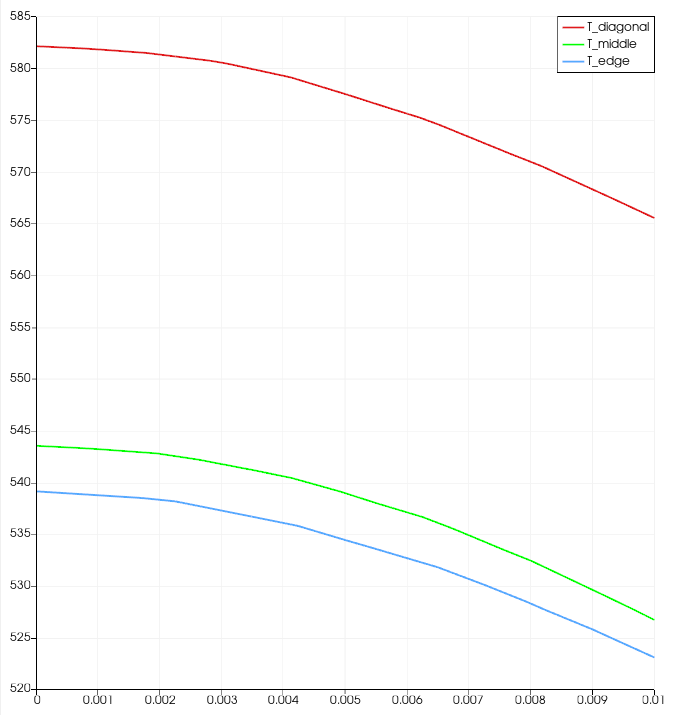
\includegraphics[width=0.4\linewidth]{6.png}
		\caption{Распределение температур в нагревателях для всех моделей} %% подпись к рисунку
	\end{center}
\end{figure}

\newpage
\par
Затем было проведено 2000 итераций расчета. Для отслеживания сходимости во время проведения расчета были построены следующие графики (пример для модели 1):
\begin{figure}[h]
	\begin{center}
		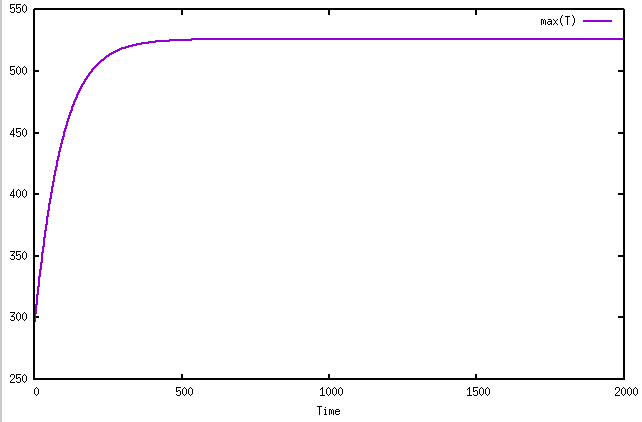
\includegraphics[width=0.35\linewidth]{11.1.png}
		\caption{Зависимость максимальной температуры радиатора от шага} %% подпись к рисунку
	\end{center}
\end{figure}
\begin{figure}[h]
	\begin{center}
		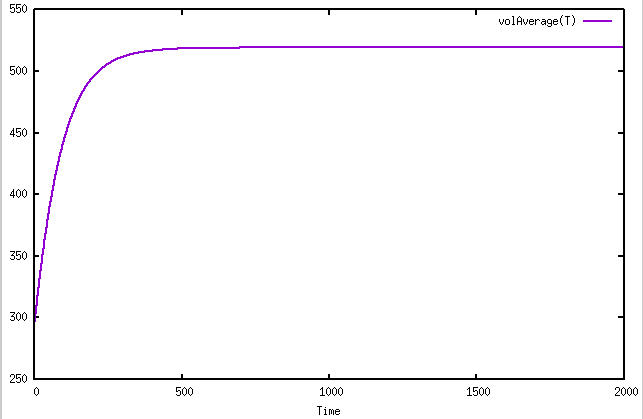
\includegraphics[width=0.35\linewidth]{12.1.png}
		\caption{Зависимость средней температуры радиатора от шага} %% подпись к рисунку
	\end{center}
\end{figure}
\begin{figure}[h]
	\begin{center}
		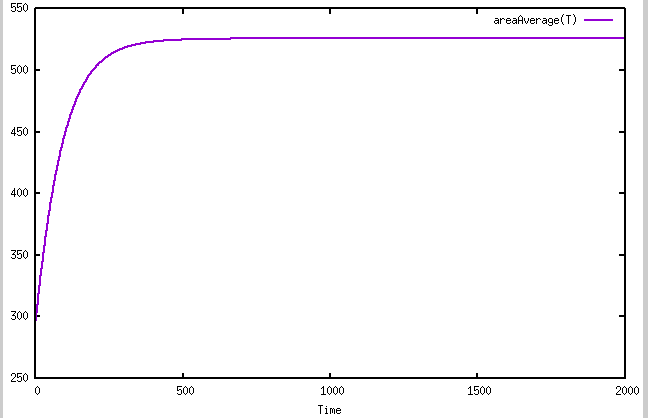
\includegraphics[width=0.35\linewidth]{13.1.png}
		\caption{Зависимость средней температуры интерфейса между нагревателем и радиатором от шага} %% подпись к рисунку
	\end{center}
\end{figure}
\newpage
\begin{figure}[h]
	\begin{center}
		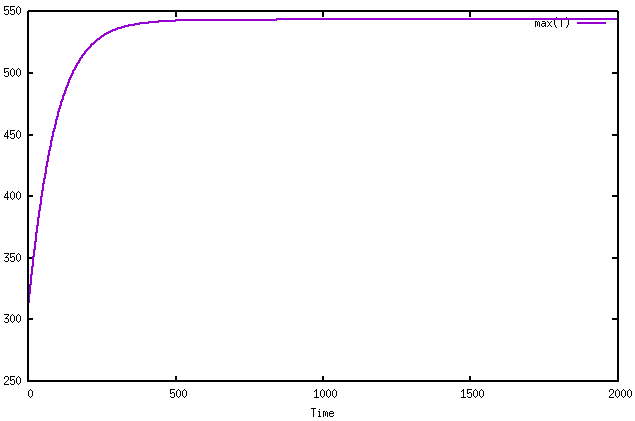
\includegraphics[width=0.4\linewidth]{14.1.png}
		\caption{Зависимость максимальной температуры нагревателя от шага} %% подпись к рисунку
	\end{center}
\end{figure}
\begin{figure}[h]
	\begin{center}
		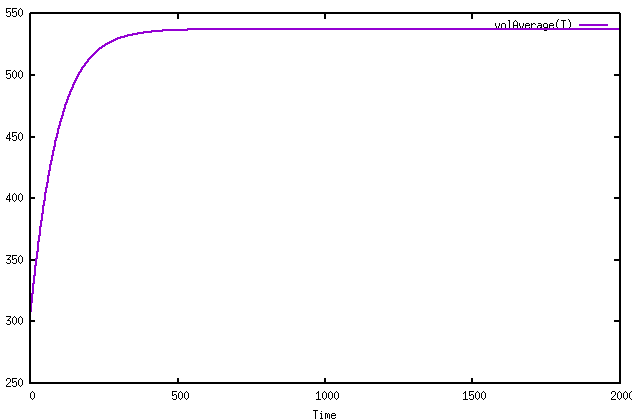
\includegraphics[width=0.4\linewidth]{15.1.png}
		\caption{Зависимость средней температуры нагревателя от шага} %% подпись к рисунку
	\end{center}
\end{figure}

\par
Далее были построены графики распределений температуры в центральном сечении:

\begin{figure}[h]
	\begin{center}
		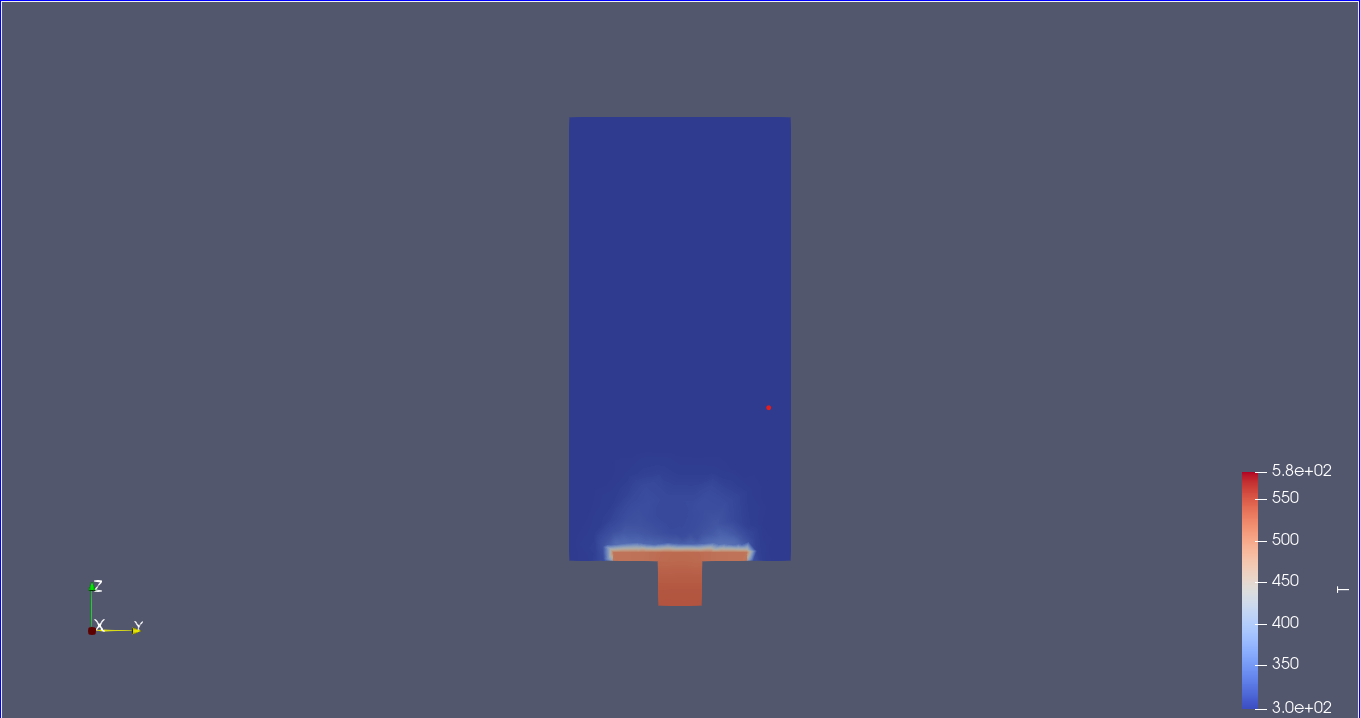
\includegraphics[width=0.4\linewidth]{7.1.png}
		\caption{Распределение температуры для модели 1} %% подпись к рисунку
	\end{center}
\end{figure}

\begin{figure}[h]
	\begin{center}
		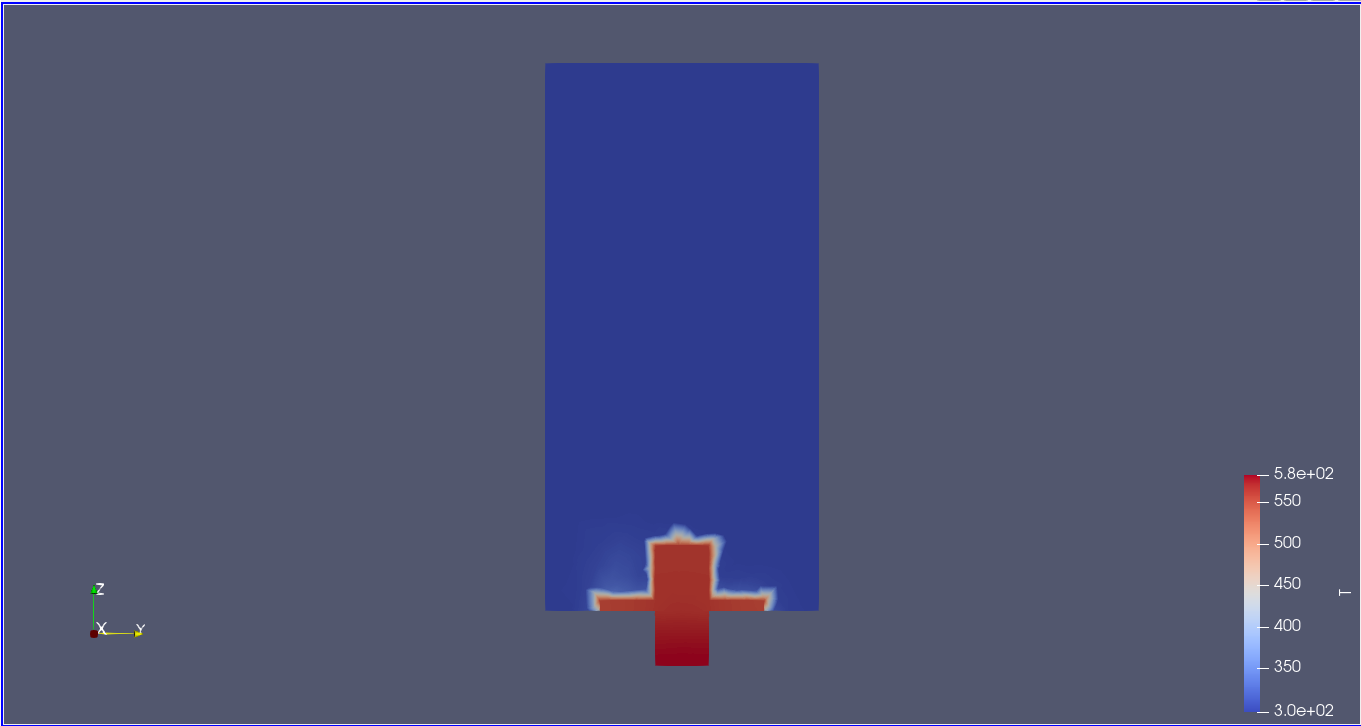
\includegraphics[width=0.4\linewidth]{7.2.png}
		\caption{Распределение температуры для модели 2} %% подпись к рисунку
	\end{center}
\end{figure}
\newpage
\begin{figure}[h]
	\begin{center}
		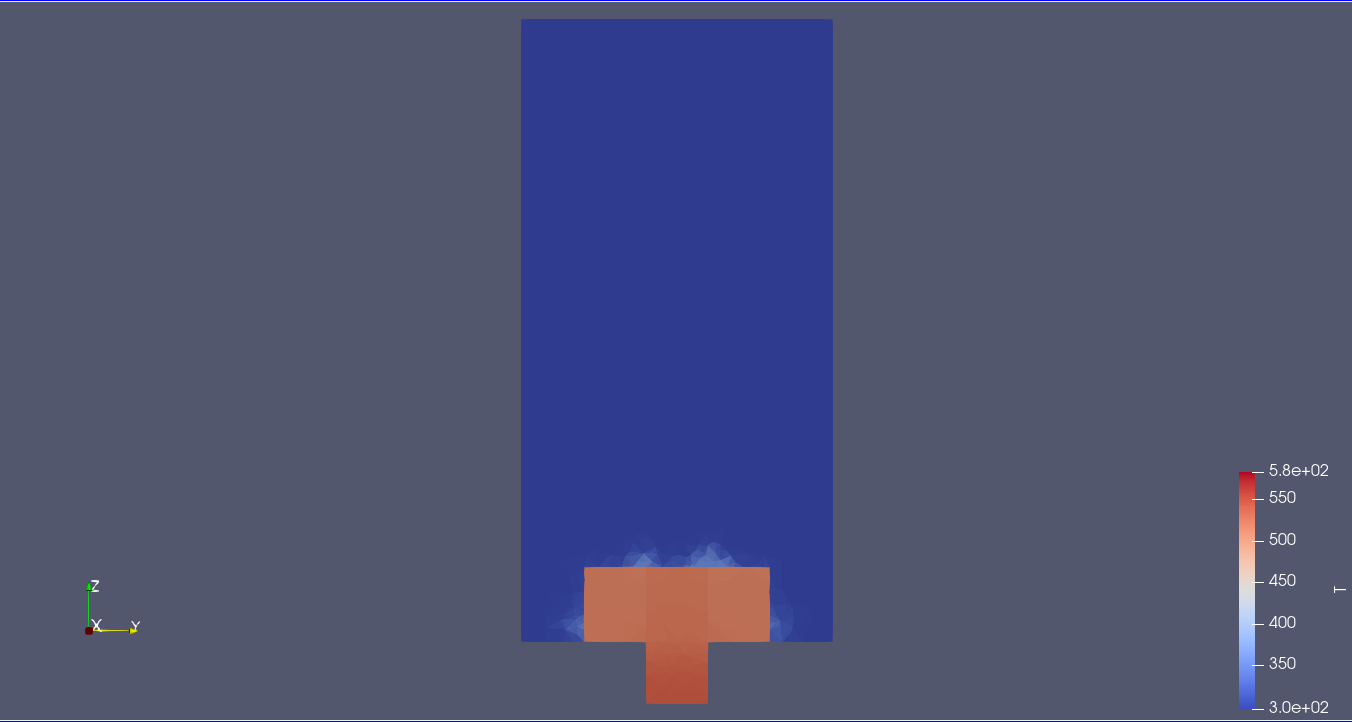
\includegraphics[width=0.4\linewidth]{7.3.png}
		\caption{Распределение температуры для модели 3} %% подпись к рисунку
	\end{center}
\end{figure}

\par
И графики распределений скоростей:
\begin{figure}[h]
	\begin{center}
		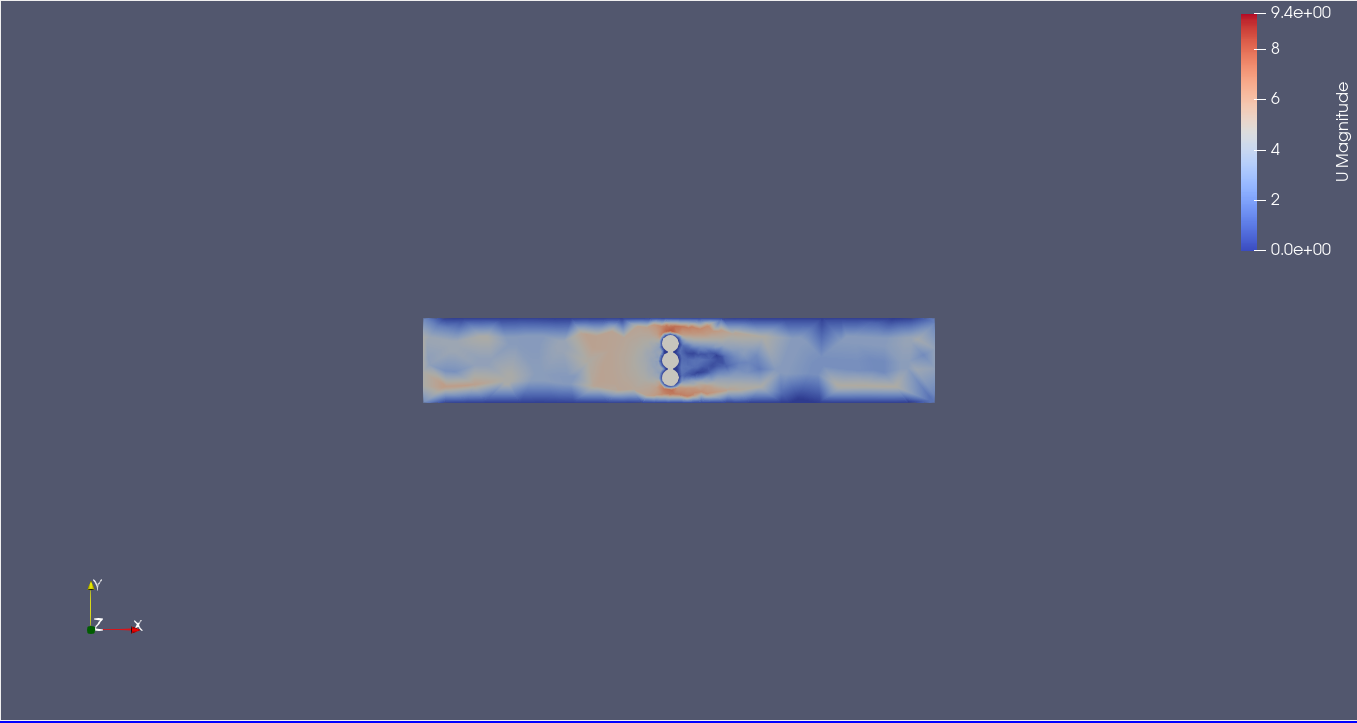
\includegraphics[width=0.4\linewidth]{8.1.png}
		\caption{Распределение скоростей для модели 1} %% подпись к рисунку
	\end{center}
\end{figure}

\begin{figure}[h]
	\begin{center}
		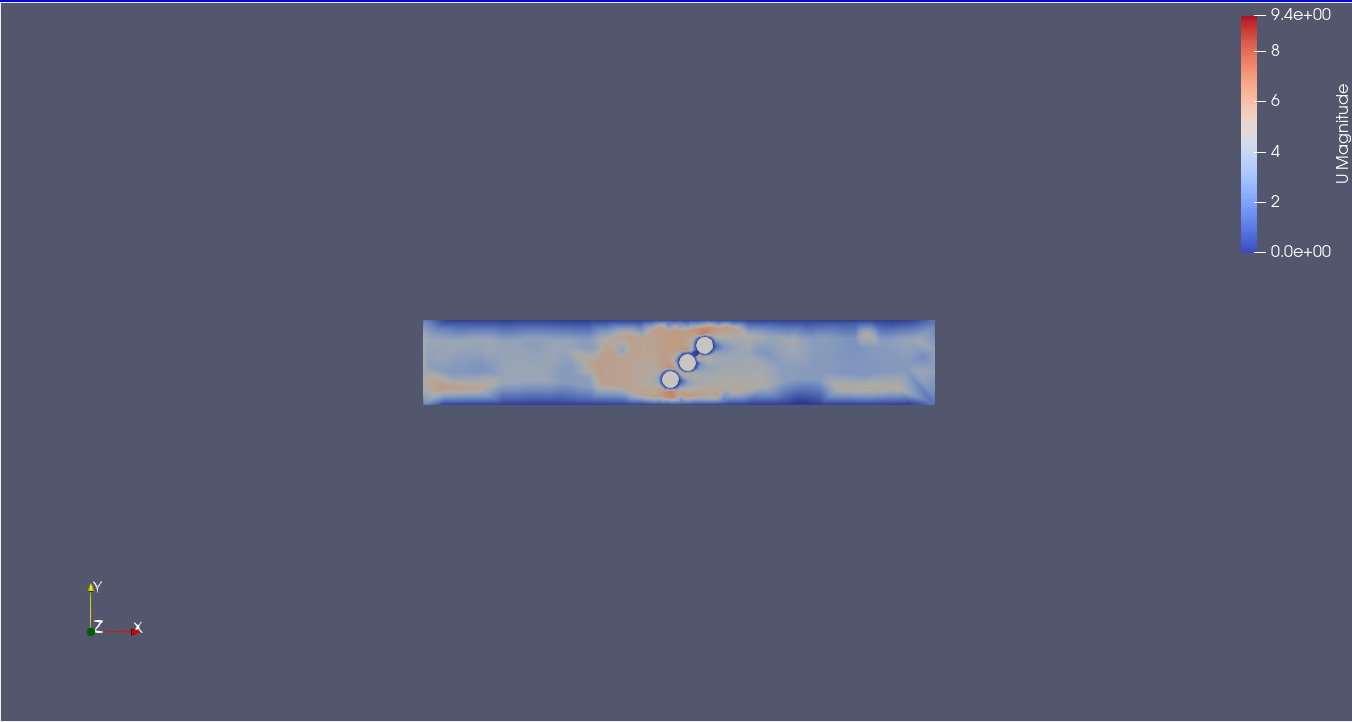
\includegraphics[width=0.4\linewidth]{8.2.png}
		\caption{Распределение скоростей для модели 2} %% подпись к рисунку
	\end{center}
\end{figure}
\newpage
\begin{figure}[h]
	\begin{center}
		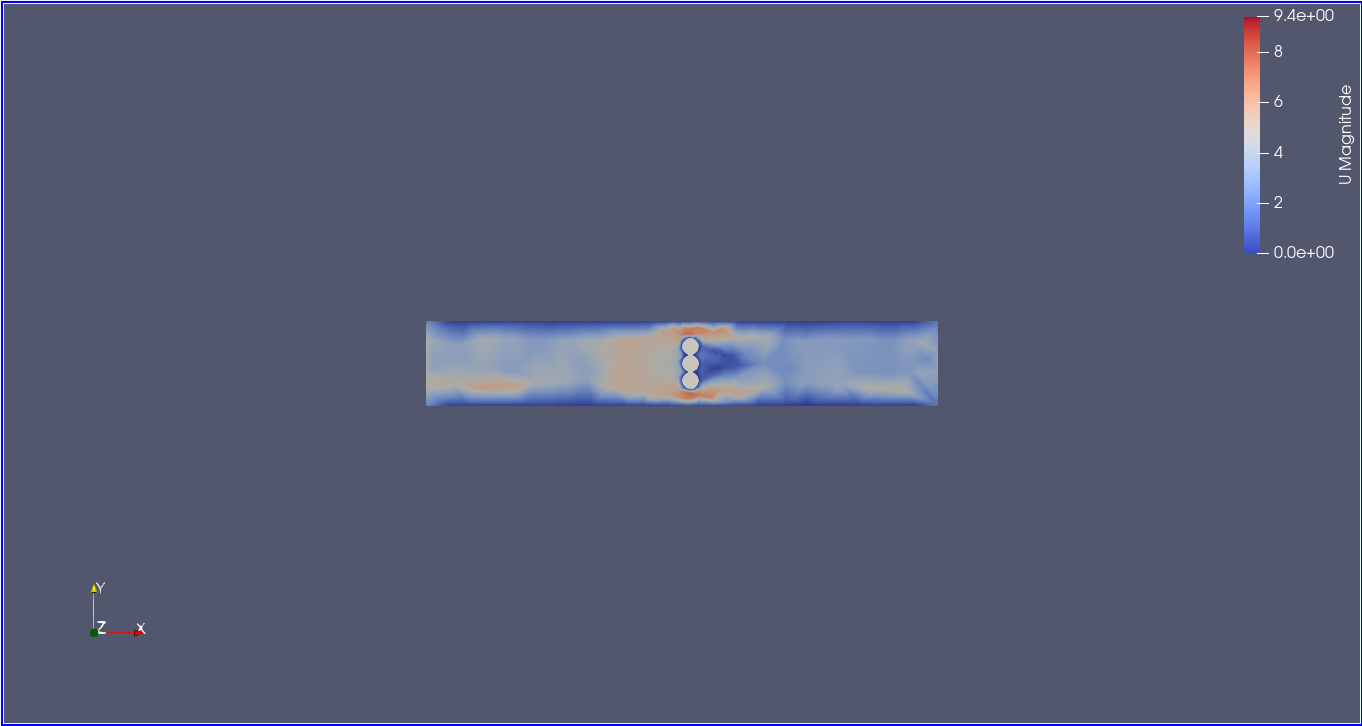
\includegraphics[width=0.4\linewidth]{8.3.png}
		\caption{Распределение скоростей для модели 3} %% подпись к рисунку
	\end{center}
\end{figure}
\begin{figure}[h]
	\begin{center}
		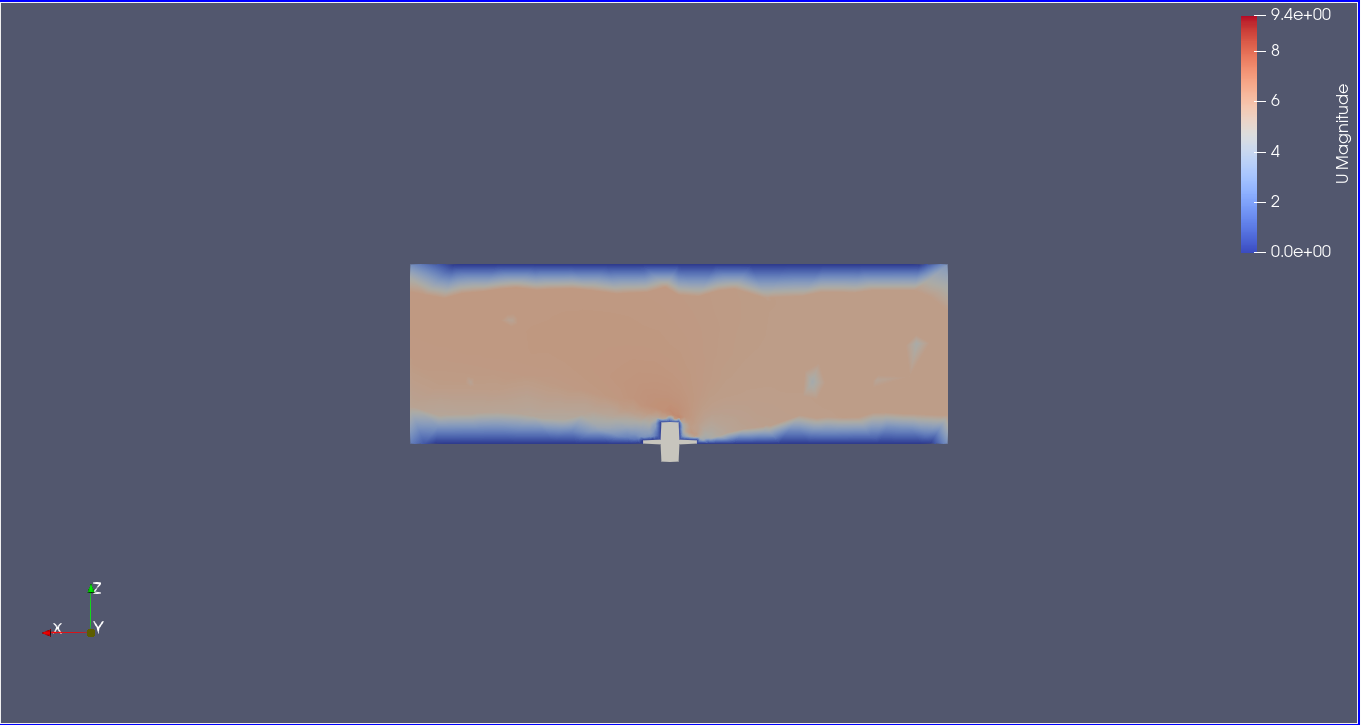
\includegraphics[width=0.4\linewidth]{9.png}
		\caption{Распределение скоростей для модели 1} %% подпись к рисунку
	\end{center}
\end{figure}

\newpage
\section{Заключение}
Результаты анализа указывают на следующие выводы: вторая модель имеет наивысшую среднюю температуру радиатора, нагревателя и интерфейса между ними, что может указывать на менее эффективное охлаждение.
Первая и третья модели демонстрируют более низкие значения средних температур радиатора, нагревателя и интерфейса.
Таким образом, основываясь на полученных результатах, можно сделать вывод о наибольшей эффективности охлаждения и лучшей теплоотдаче в первой модели, где наблюдается наименьшая средняя температура нагревателя, указывающая на более эффективную передачу тепла.
Результаты исследования подтверждают, что форма радиатора влияет на его эффективность и теплоотдачу. Модель 1 с определенным распределением цилиндров обеспечивает наилучшие результаты в задаче охлаждения нагретого тела.
Данный результат связан с тем, что форма и расположение цилиндров в модели 1 позволяют более равномерно распределить тепловую нагрузку и обеспечить эффективное охлаждение, поскольку цилиндры имеют прямой контакт между собой.
Во второй модели, где отсутствует касание между цилиндрами, наблюдается наихудший результат среди рассмотренных моделей.

\newpage
\bibliographystyle{utf8gost705u}  %% стилевой файл для оформления по ГОСТу
\bibliography{Overview}     %% имя библиографической базы (bib-файла) 

\newpage
\section{Приложение А}
% \renewcommand{\thesection}{\Asbuk{section}}
Проект можно найти на github (github.com/AlexEsn/FOAM\_project), где содержатся все скрипты и кейсы.

\newpage
\section{Приложение Б}
% \renewcommand{\thesection}{\Asbuk{section}}
В процессе работы был найден баг в SALOME-9.9.0: при дампе Python скрипта с сеткой создается файл с ошибкой.

\begin{figure}[h]
	\begin{center}
		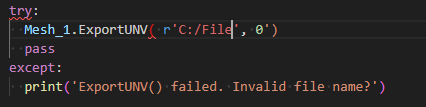
\includegraphics[width=1\linewidth]{e.png}
		\caption{Ошибка экспорта сетки} %% подпись к рисунку
	\end{center}
\end{figure}

Для её решения достаточно удалить лишние символы:
\begin{figure}[h]
	\begin{center}
		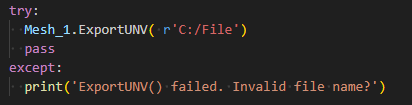
\includegraphics[width=1\linewidth]{er.png}
		\caption{Решение ошибки экспорта сетки} %% подпись к рисунку
	\end{center}
\end{figure}


\end{document}